\chapter{Introduction to the nonperturbative renormalization techniques}

At the so-called Lifshitz critical point, three phases intersect. This is rather unsual, so we expect the physics of the vicinity of this point to be of special interest. To investigate it, we would like to compute the critical exponents associated to this transition point. To this end, we used the powerful machinery of the renormalization group, and more precisely of one particular implementation of the renormalization ideas: the nonpertubative renormalization group.

In this chapter we propose first a very general introduction to the ideas and concepts of renormalization. Then we focus on the nonperturbative renormalization group techniques.

\section{Introduction to the renormalization group}

\subsection{The renormalization procedure}

The idea of renormlization is to consider a given many-body system at different length scales. At a given length scale $S$ the system is described by an effective Hamiltonian $H_S$. 
For a many-body system, two length scales play a special role: 
\begin{itemize}
\item The microscopic length scale, $a$, which is for example for a cristal the typical distance between two neighbouring atoms.
It is convenient to define the scale in the units of the microscopic lenghtscale $a$, and this is what we are going to do. So, for example, the system at $S=3$ will mean the system at lengthscale $3 a$.
\item The macroscopic length scale $L$, which is the size of the system. 
\end{itemize}

The Hamiltonian at the microscopic length scale is simply the microscopic Hamiltonian, \textit{ie}
\begin{equation}
H_1 = H
\end{equation}
 while the Hamiltonian at the macroscopic length scale is called to effective action (and sometimes the Gibbs free energy) and is denoted $\Gamma$:
\begin{equation}
  H_{L/a} = \Gamma
\end{equation} 

For the moment what we mean by ``the Hamiltonian at a length scale $S$'' is rather vague. To be more precise, let us imagine that we want to describe a magnetic cristal. The microscopic Hamiltonian will be in general a discrete sum of local observables $O_\alpha$, depending on the value of the magnetization at site $i$, $\phi(i)$:
\begin{equation}
H[\phi] = \sum_i \sum_\alpha \kappa_\alpha O_\alpha[\phi(i), \nabla \phi(i), ...]
\end{equation}
where $\kappa_\alpha$ is the coupling constant associated to the observable $O_\alpha$. The partition function will be simply the sum over all possible configurations of the $\phi(i)$ of the Boltzmann weight associated to a given configuration:
\begin{equation}
Z = \sum_{\text{conf } \phi} e^{-H[\phi]}
\end{equation}
These equations describe the system at the microscopic scale $S=1$. Now, if we want to describe it at a scale $S \geq 1$, surely we are no longer interested in knowing the fluctuations of the field over regions of size smaller than $a S$\footnote{Experimentally, we can imagine that looking at the system at scale $S$ means probing it with devices having a spatial resolution of $a S$. Any measurement operation with such devices can be described mathematically by the convolution of an observable by an error function having a spatial support of diameter $a S$. This operation is roughtly equivalement to averaging the observables (and therefore the field) on blocks of size $a S$.}. All we need is thus the average over regions of size $a S$ of the field:
\begin{equation}
\tilde{\phi}(b) = \frac{1}{(aS)^d} \sum_{i \in B(b)} \phi(i)
\end{equation}
where $d$ is the dimension of space, and $B(b)$ is the set of sites $i$ belonging to the block $b$.

Schematically what we do is group spins by blocks of size $a S$ (fig. \ref{renorm_1}), and average over these blocks.

\begin{figure}[htp]
\centering
\begin{subfigure}{.25\textwidth}
	\centering
	
\includegraphics[width=.9\linewidth]{img/chap2/renorm_step0.pdf}
	\caption{The initial lattice.}
	\label{renorm_0}
	\end{subfigure}%
\begin{subfigure}{.25\textwidth}
	\centering
	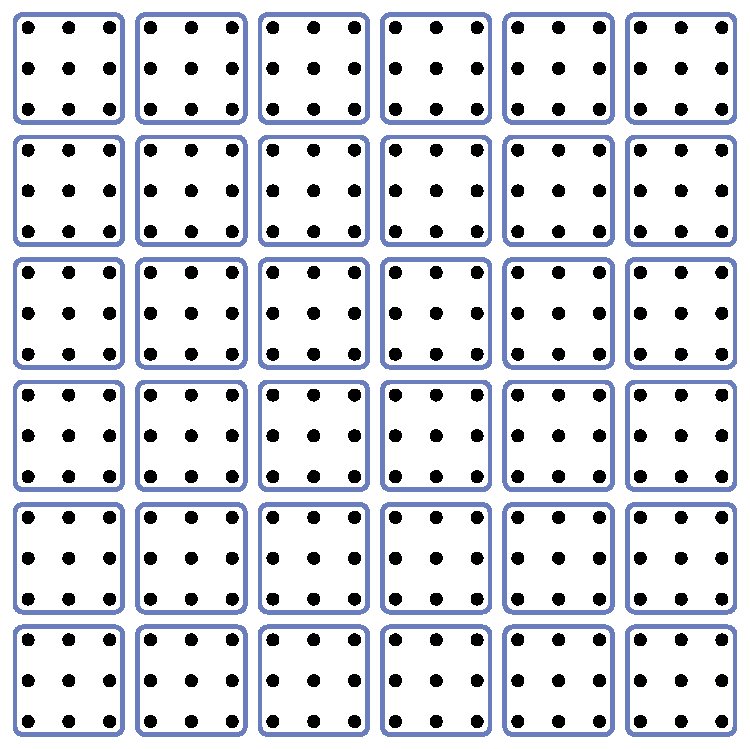
\includegraphics[width=.9\linewidth]{img/chap2/renorm_step1.pdf}
	\caption{Block spin averaging.}
	\label{renorm_1}
\end{subfigure}%
\begin{subfigure}{.25\textwidth}
	\centering
	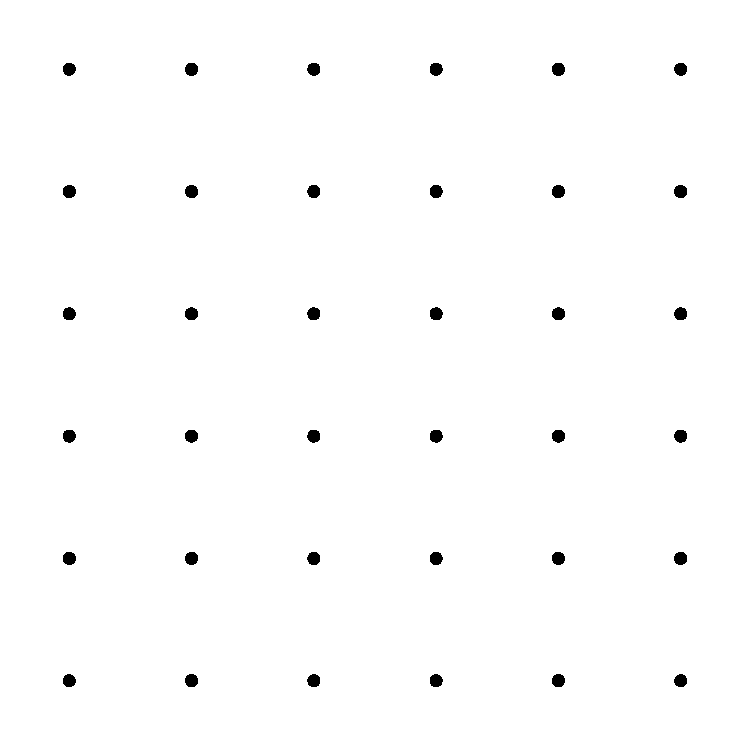
\includegraphics[width=.9\linewidth]{img/chap2/renorm_step2.pdf}
	\caption{The new lattice.}
	\label{renorm_2}
\end{subfigure}%
\begin{subfigure}{.25\textwidth}
	\centering
	
\includegraphics[width=.9\linewidth]{img/chap2/renorm_step3.pdf}
	\caption{Rescaling.}
	\label{renorm_3}
\end{subfigure}
\caption{The renormalization procedure illustrated. Here we have chosen $S = 3$.}
\label{fig:renorm_proc}
\end{figure}

Now we replace the microscopic Hamiltonian by an effective Hamiltonian for the block spin field $\tilde{\phi}$:
\begin{equation}
\label{eq:effective_ham}
H[\phi] \rightarrow \tilde{H}[\tilde{\phi}] \text{ such that } e^{-\tilde{H}[\tilde{\phi}]} = \sum_{\text{conf } \phi} \prod_{b} \delta \left( \tilde{\phi}(b) - \frac{1}{S^d} \sum_{i \in B(b)} \phi(i) \right) e^{-H[\phi]}
\end{equation}
this Hamiltonian is designed such that
\begin{equation}
\sum_{\text{conf } \tilde{\phi}} e^{-\tilde{H}[\tilde{\phi}]} = Z
\end{equation}
This Hamiltonian describe the new system depicted in fig. \ref{renorm_2}. 
We are not done yet! To make the new Hamiltonian ressemble as much as possible the one we started from, we rescale all lengths (fig. \ref{renorm_3}). We also rescale the field. Formally it means that we perform the change of variables
\begin{eqnarray}
x' = x/S  \\
\phi' = S^\Delta \tilde{\phi}
\end{eqnarray}
where $x$ could be any length appearing in the Hamiltonian.

The Hamiltonian in the new variables $H'[\phi'] = \tilde{H}[\tilde{\phi}]$ is the effective Hamiltonian after the renormalization operation.  
It could seem strange that we rescaled the field as well as the lenghts. We do that in order for the new Hamiltonian to ressemble the old one as closely as possible. We are going to see on the example of the Lifshitz mean field theory how we can chose $\Delta$ for that purpose.

To conclude, the key ideas of the renormalization procedure are the averaging over block spins, and the rescaling of lengths and fields. We have described here the case of a discrete Hamiltonian, because it seemed more intuitive. But of course the ideas of renormalization are general and can as easily be applied to a continuous Hamiltonians.

\subsection{The renormalization group}

If the structure of the Hamiltonian is kept unchanged by the renormalization group procedure, \textit{ie} if
\begin{equation}
H'[\phi'] = \sum_{i'} \sum_\alpha \kappa_\alpha' O_\alpha[\phi'(i'), \nabla' \phi'(i'), ...]
\end{equation}
then the renormalization group action is a group action\footnote{Actually, invertibility cannot be guaranteed so it rather is a semigroup action, but the distinction is of no importance for us.}. The group renormalization group is completely described by its action on the coupling contants:
\begin{equation}
\kappa_\alpha \rightarrow \kappa_\alpha' \define g(\kappa_\alpha, S)
\end{equation}
The renormalization group is a multiplicative, one parameter group:
\begin{equation}
g( g(\kappa_\alpha, S_1), S_2) = g(\kappa_\alpha, S_1 S_2)
\end{equation}
These transformations are assumed to be continuous in the coupling constant. It is also very often possible to consider the scale $S$ as a continuous parameter. Then the successive application of infintesimally close renormalization group transformations generates a continuous tranjectory in the space of coupling constants. This trajectory can be parametrized by $t \define \log(S)$, an additive parameter playing the role of a time. It is often referred to as ``the renormalization group time''.

Near a phase transition or critical point, fluctuations occur at all length scales, and thus one should expect the Hamiltonian to be scale invariant. 
In terms of the renormalization group action, scale invariance simply means that
\begin{equation}
g(\kappa_\alpha, S) = \kappa_\alpha
\end{equation}
The fact that scale invariance has such a simple meaning in the renormalization group framework is an extremely good sign. It is a hint that renormalization group is a powerful tool to look for critical points.

To illustrate that, in appendix ??? (yet to be written!), we derive from very simple renormalization group arguments some useful formulas relating critical exponents.

\subsection{Renormalization procedure applied to the mean field Lifshitz theory}

As we have just seen, an operation from the renormalization group transforms our microscopic Hamiltonian $H$ into an effective Hamiltonian at scale $S$, $H_g(S)$. We hope that this operation will not change the structure of our Hamiltonian, so that we can use the tools of the renormalization group. 
Since our Hamiltonian is not isotropic (it distinguishes between the direction of the modulation $\sslash$, and the orthogonal direction $\perp$), we expect an operation of the renormalization group to change lengthscales by two different amounts in the two unequivalent directions. 
Scales in the parallel direction will be changed by a factor $S_\sslash$
 : $x_\sslash' = (S_\sslash)^{-1} x_\sslash$
, while scales on the orthogonal direction will be changed by a factor $S_\perp$ : $x_\perp' = (S_\perp)^{-1} x_\perp$.

To simplify things we can keep a single scale $S = S_\perp$, and define $\theta$ such that $S_\sslash = S^\theta$.Note that this is equivalent to changing the \textit{units} in the parallel direction: if we say that lengths in the orthogonal direction are measured in meters, then lengths in the parallel direction are measured in $(\text{meters})^\theta$.
A volume, which is normally measured in $(\text{meters})^d$ will in our new units system be measured in $(\text{meters})^{(d-m) + \theta m}$. It is as if $d$ had been replaced by
\begin{equation}
d_m = d+ m(\theta -1)
\end{equation}

We define two anomalous dimensions by
\begin{align}
\langle \phi(p_\sslash) \phi(0) \rangle_{g^*} \propto |p_\sslash|^{\eta_\sslash -4} \\
\langle \phi(p_\perp) \phi(0) \rangle_{g^*} \propto |p_\perp|^{\eta_\perp -2} 
\end{align}
where $g^*$ is a fixed point in the space of coupling constants, and the proportionality constant is independent of the scale.

But we also know that
\begin{align}
\langle \phi(p_\sslash) \phi(0) \rangle_{g^*} \propto |p_\sslash|^{\frac{2 \Delta}{\theta}} \\
\langle \phi(p_\perp) \phi(0) \rangle_{g^*} \propto |p_\perp|^{2\Delta} 
\end{align}
where $\Delta$ is the renormalization of the field : $\phi_{g(1)}(x) = S^{-\Delta} \phi_{g(S)}(Sx)$. 
Identifying these expressions for the renormalization of the correlation function with the previous ones, we can express $\Delta$ in two unequivalent ways, thus yielding a relation between $\eta_\sslash$ and $\eta_\perp$ :
\begin{equation}
\theta = \frac{2- \eta_\perp}{4- \eta_\sslash}
\end{equation}

\subsubsection{Mean field analysis}

We recall that the Lifshitz Hamiltonian is
\begin{equation}
H = \int_x \left( \frac{1}{2}(\partial_\perp \phi)^2 + \frac{\rho_0}{2} (\partial_\sslash \phi)^2 + \frac{\sigma_0}{2} (\partial_\sslash^2 \phi)^2 + U(\rho) \right)
\end{equation}

The mean field approximation consist in neglecting the fluctuations of the field. Therefore, the integration over the fluctuations performed during a renormalization group operation is trivial, and we can directly write the transformed Hamiltonian after a renormalization group operation $g(S)$ :
\begin{equation}
H'[\phi'] = \int_{x'} S^{d_m} \left( S^{-2\Delta -2} (\partial_\perp' \phi')^2 + \sigma_0 S^{-2\Delta - 4 \theta} (\partial_\sslash'^2 \phi)^2 + \rho_0 S^{-2\Delta -2 \theta} (\partial_\sslash' \phi')^2 U'(\phi') \right)
\end{equation}
This Hamiltonian must indentify with the previous one, so
\begin{equation}
\Delta = \frac{d_m -2}{2}
\end{equation}
The Lifschitz point involves a non-trivial $\sigma_0 (\partial_\sslash^2 \phi)^2$, therefore at this critical point, $\sigma_0$ must not renormalize away, which is only possible if
\begin{equation}
\theta = \frac{1}{2}
\end{equation}

In the mean field approximation, it is as if the physical dimension were
\begin{equation}
d_{\text{mean field}} = d - \frac{m}{2}
\end{equation}
We immediately deduce that the upper critical dimension\footnote{The upper critical dimension is the dimension above which mean field theory is exact, in the sense that it gives the correct critical exponents.}, which is ``normally'' 4, becomes
\begin{equation}
d_c^> = 4 + \frac{m}{2}
\end{equation}
around the Lifschitz point.

In nature, the most common case is $m=1$ (when in the modulated phase, the field is periodic in one direction of space). In that case the upper critical dimension is $d_c^> = 4.5$. When doing perturbation theory, one usually expand around the upper critical dimension, writing
\begin{equation}
d = d_c^> - \epsilon,
\end{equation} 
where $\epsilon$ is a supposedly small parameter. When $d=3$, $\epsilon = 1.5$, which is not so small. So we expect the results from perturbation theory to be rather imprecise. To better tackle this problem, it would be great to have a method that is not perturbative in the dimension. This is what the nonperturbative renormalization group method provides, as we will now see.

\section{The nonperturbative renormalization group}

Starting from the microscopic Hamiltonian $H$, and applying successive transformations of the renormalization group, we construct a hierarchy of effective Hamiltonian describind the system at greater and greater distances. This process come to an end when we describe the system at the macroscopic distance. We then obtain the effective action $\Gamma$.
\begin{equation}
H \rightarrow H' \rightarrow H'' \rightarrow ... \rightarrow \Gamma
\end{equation}
Writing primes is cumbersome, so we devise a better notation system. We call $H_k$ the effective Hamiltonian describing the system at lengthscale $1/k$. Then our previous hierarchy reads
\begin{equation}
H_\Lambda \rightarrow H_{\Lambda - \delta k} \rightarrow H_{\Lambda - 2 \delta k} \rightarrow ... \rightarrow H_0
\end{equation}

The idea of the nonperturbative renormalization group is to consider $H_k$ \textit{as a function of $k$}. We already know the boundary values $H_\Lambda$ and $H_0$. If we could find a differential equation on $H_k$, it would be entirely determined!

Many exact differential equations can be derived from this starting point. They lead to different version of the nonperturbative renormalization group. We shall discuss here the so-called Wetterich, or Wegner-Wetterich equation, whose object of study is not the scale-dependent Hamiltonian but the scale dependent \textit{effective action} at scale $k$,  $\Gamma_k$. The effective action $\Gamma$ takes into account fluctuations on all length scales (ie on all momentum scales), while $\Gamma_k$ only takes into account fluctuations of momentum between $k$ and $\Lambda$.

\subsection{The scale-dependent effective action}

\begin{figure}[htp]
\begin{center}
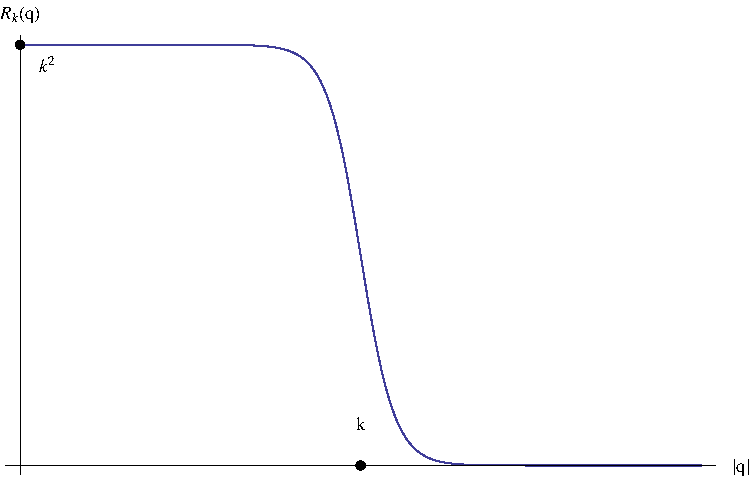
\includegraphics[scale=0.7]{img/chap2/regulator.pdf}
\caption{Typical shape of the regulator function in momentum space $R_k(q)$.}
\label{fig:regulator}
\end{center}
\end{figure}

Let us try to build $\Gamma_k$ explicitely.  To this end let us define the \textit{regulator} $R_k(x,y) = R(x) \delta(x-y)$, whose role is to give a mass to the modes of momentum smaller than $k$, while leaving the other modes untouched.
The typical shape of the regulator in momentum space is given by fig. \ref{fig:regulator}. Moreover, the regulator is required to vanish at $k \rightarrow 0$ and to diverge for $k \rightarrow \infty$ (or $k \rightarrow \Lambda$), at fixed $q^2$. This can for example be achieved by
\begin{equation}
R_k(q) = \frac{q^2}{e^{q^2/k^2} - 1}
\end{equation}

We now introduce a modified, scale dependent Hamiltonian:
\begin{equation}
H_k[\varphi] \define H[\varphi] + \Delta H_k[\varphi], \text{~with~} \Delta H_k[\varphi] \define \frac{1}{2} \varphi \cdot R_k \cdot \varphi = \frac{1}{2} \int_{x,y} \varphi(x) R_k(x,y) \varphi(y)
\end{equation}

We see that the $\Delta H_k$ term is a quadratic on the field. Thus $R_k$ indeed acts as a scale-dependent and momentum-dependent squared mass term, giving a mass of order $k^2$ to the ``slow'' modes of momentum smaller than $k$.

We can now define the Legendre transform of the scale dependent free energy,
\begin{equation}
\label{eq:gamleg}
\gamleg[\phi] \define - W_k[h] + h \cdot \phi
\end{equation}
where the free energy is defined as $W_k[h] = \log Z_k$, and $Z_k = \int \D \varphi e^{-H_k[\varphi] + h \cdot \varphi} $.
Qualitatively, since the slow modes are given a mass in $W_k$, the Legendre transform only acts on the rapid mode, and we understand that  $\gamleg[\phi]$ indeed has the property of taking into accounts only rapid modes.\footnote{We note in passing that eq. \ref{eq:gamleg} implies 
\begin{equation}
\phi(x) = \frac{\delta W_k[h]}{
\delta h(x)} = \frac{1}{Z_k[\varphi]} \int \D \varphi e^{-H_k[\varphi] + h \cdot \varphi} \varphi \define \langle \varphi(x) \rangle_k
\end{equation}
This tells us that $\phi$ is the background field (at scale $k$), \textit{ie} the mean value of the field $\varphi$ (at scale $k$). }

Finally, we introduce the scale-dependent effective action:
\begin{equation}
\gam_k[\phi] \define \gamleg[\phi] - \Delta H_k[\phi]
\end{equation}
This object has the right properties to be the effective action at scale $k$. Indeed it can be shown to verify $\gam_0 = \Gamma$, $\gam_\Lambda = H$.\footnote{The first identity is trivial, given the properties of the regulator function. Proving the second one requires slightly more work. It can be shown using that $\exp{-\Gamma_k[\phi]} = \int \D \varphi \exp{-S[\varphi] + \frac{\delta \Gamma}{\delta \varphi} \cdot (\varphi - \phi) - \frac{1}{2} (\varphi - \phi ) \cdot R_k \cdot (\varphi - \phi) }$, and remembering that $R_k \rightarrow \infty$ when $k \rightarrow \Lambda$.}


Finally, the scale-dependent effective action verifies the differential equation
\begin{equation}
\p{k} \gam_k[\phi] = \frac{1}{2} \int_{x,y} \p{k}\left(R_k(x,y)\right) \left( \Gamma^{(2)}_k(x,y) + R_k(x,y) \right)^{-1}
\end{equation}
This equation is often called the Wetterich equation. 
The demonstration can be found in appendix \ref{app:wett}. We can use the fact that $R_k$ is invariant by translation, to write the right hand side of this integro-differential equation as a single integral over momentum $q$:
\begin{equation}
\p{k} \gam_k[\phi] = \frac{1}{2} \int_{q} \p{k}\left(R_k(q)\right) \left( \Gamma^{(2)}_k(q,-q) + R_k(q) \right)^{-1}
\end{equation}
Moreover, we shall make the change of variable $k \rightarrow t = \log(k/\Lambda)$, to take advantage of the additive properties of $t$\footnote{As we have seen before, $t$ can be regarded as a time parameterizing the renormalization group trajectory in the coupling constants space.}. In order to simplify further the Wetterich equation, we define an operator $\hat{\p{t}}$ as the differenciation with respect to $t$ acting only on $R_t$. That is,
\begin{equation}
 \hat{\p{t}} \define \frac{\partial R_t(\fdot)}{\partial t} \frac{\partial}{\partial R_t(\fdot)}
\end{equation}
where $R_t(\fdot)$ is a shorthand notation for the function $q \mapsto R_t(q)$. 
 We have then
\begin{equation}
\label{eq:wett}
\p{t} \gam_k[\phi] = \frac{1}{2} \hat{\p{t}} \tr{ \log\left( \Gamma^{(2)}_t(q,-q) + R_t(q) \right) }\footnote{Here we have used the formula for the trace on continuous indices in Fourier space: $\tr{A} = \int_{x} A(x,x) = \int_q A(q,-q)$.}
\end{equation}
This is the form of the Wetterich equation we will use from now on. 
Even if the field is vectorial, eq. \ref{eq:wett} is still valid, provided that the trace acts on the vector space of the field as well\footnote{we refer to appendix \ref{app:wett} for a sketch of proof}.

Note that no approximations were made in the course of deriving the Wetterich equation. It is thus an exact equation describing the (renormlization group) time dependance of the scale-dependant effective action $\Gamma_t$, interpolating between $\Gamma_\Lambda = H$ and $ \Gamma_0 = \Gamma$.

We we can use the Wetterich equation as a starting point for finding the critical properties of the Lifshitz model.